
%mainfile: Behavior_modeling.tex

\pagestyle{fancy} 
\lhead{Atelier Nueromodélisation, 2017}
\rhead{Problem set \#2}
\rfoot{\thepage}
\cfoot{}
\lfoot{~\theauthor}
\renewcommand{\headrulewidth}{0.4pt}
\renewcommand{\footrulewidth}{0.4pt}


\title{Problem Set \#2: Quantitative Models of Behavior \vspace{-0.5em}}
%\preauthor{} \postauthor{} 
\author{Hsieh Yu-Guan}
\date{\today}
\maketitle

\thispagestyle{fancy}


\section*{Introduction}

In this report we will work on several classic behavior models. The topics 
that we will cover include conditional learning (classical conditioning and
operant conditioning), decision making and reinforcement learning.


\section{Rescola-Wagner model}

\subsection{Model description}

Let's start with the Rescola-Wagner model. It's a model of classical
conditioning in which learning signifies building associations between 
conditioned (CS) and unconditioned (UCS) stimuli. UCS are often represented in
form of rewards like food (for an animal) or money (for a person) while CS are 
some kinds of neutral stimuli that may or may not allow us to predict the
occurrence of this reward.

In a single trial, the presence or absence of the reward is respectively 
denoted by $r = 0$ or $r = 1$. More than one CS can be taken into account, 
then the presence of the $i^{th}$ stimulus is denoted by $u^{(i)} = 1$ and its 
absence by $u^{(i)} = 0$. The animal's prediction $v$ is given by the 
formula

\[v = \sum_{i = 1}^m w^{(i)}u^{(i)}\]

\noindent
where $m$ is the number of CS, and for each $i$, $w^{(i)}$ is the prediction 
parameter associated with $u^{(i)}$. If we note $u = (u_1, ..., u_m)$ and 
$w = (w_1, ..., w_m)$, it can also be written in the form 

\[v = w\cdot u\]

\noindent
where $\cdot$ denotes the scalar product. We can now calculate the predition
error $\delta = r - v$ which, with the learning rate $\epsilon$, allows us to
write down the update rule for every $w^{(i)}$ after the trial at time $t$

\[w_{t+1}^{(i)} = w_t^{(i)} + \epsilon\delta_t u_t^{(i)}.\]


\subsection{A simple test}

To examine the reliability of the model, we'll first look at a very simple
experiment. Only one stimulus is considered, so we identify for the moment
$u$ with $u^{(1)}$ and $w$ with $w^{(1)}$. Let's assume that in the first 25 
trials, both stimulus and reward are present, and during the next 25 
trials, only the stimulus is present. The plot of $r$ and $u$ is shown in 
the figure below.

\vspace{-1em}
\begin{figure}[H]
  \centering
  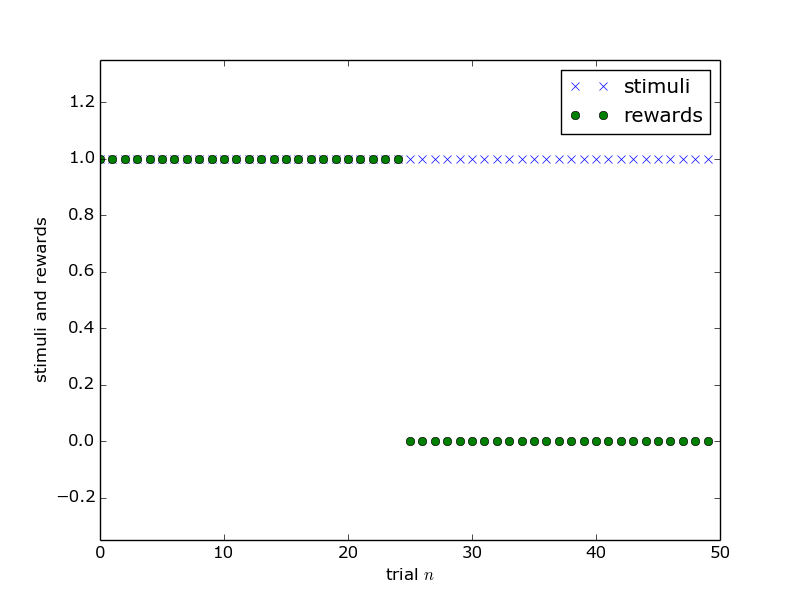
\includegraphics[width=0.7\linewidth]{pavCond1}
  \caption{A very simple experiment}
\end{figure}

Now if we do the simulation with the learning rate $\epsilon = 0.1$, the value 
of $w$ evolves as shown (since $u$ equals always 1 here, we have also all the 
time $v = w$).

\vspace{-1em}
\begin{figure}[H]
  \centering
  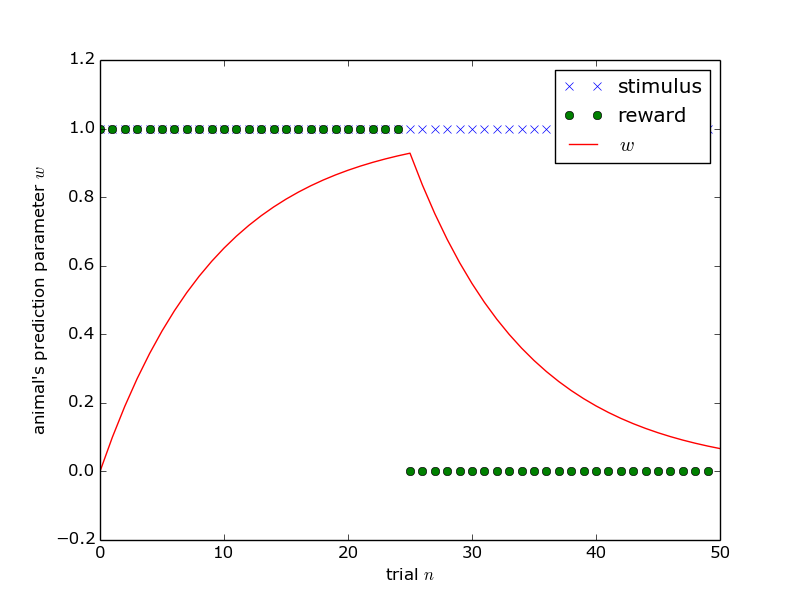
\includegraphics[width=0.7\linewidth]{pavCond2}
  \caption{Evolution of $w$ in this simple experiment ($\epsilon = 0.1$)}
\end{figure}

We see an exponential rise of $w$ to value 1 during the first 25 trials and 
its value decays exponentially to 0 for the rest of the experiment. It's 
rather reasonable intuitively, and from a mathematical point of view, we 
write simply $w_{t+1} - w_t = \epsilon\delta_t u_t$. We know that 
$\delta_t = r_t - w_t$ (remember that $v_t = w_t$ here) and $u_t = 1$ for all 
$t$. For the first 25 trials, we get $w_{t+1} - w_t = \epsilon(1 - w_t)$, so
if we put it in a continuous form, it becomes 

\[\frac{dw}{dt} = \epsilon(1-w).\]

\noindent
We now just need to solve this differential equation to see that 
$w_t = 1 - e^{-\epsilon t}$. In the same way, for the trials 26 to 50,
we can get $w_t = Ae ^ {-\epsilon(t-25)} $ where $A$ is a constant that can be
decided given a particular value of $w_t$. 

The next thing to do is surely to
study the impact of the learning rate, so we vary the value of $\epsilon$.

\vspace{-1em}
\begin{figure}[H]
  \centering
  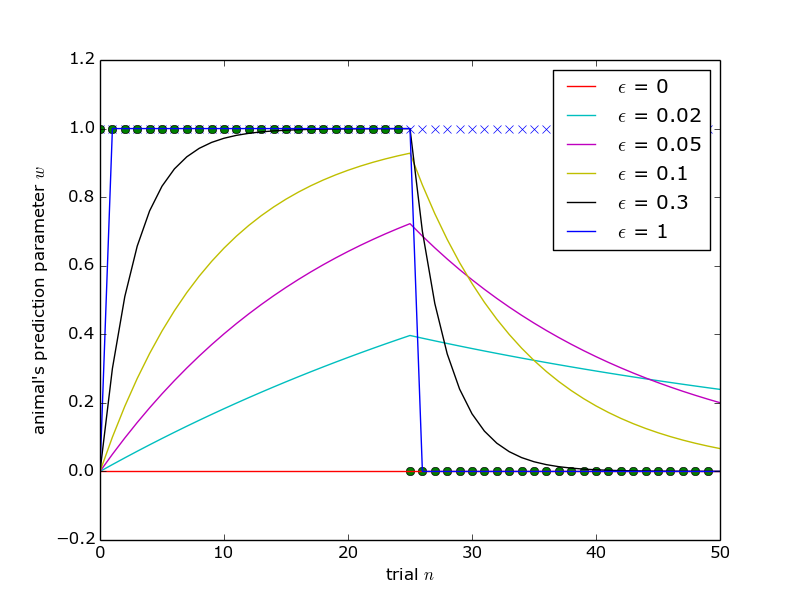
\includegraphics[width=0.7\linewidth]{pavCond3}
  \caption
    {Evolution of $w$ in the same experiment but with different $\epsilon$}
\end{figure}

As what our formula implies, greater the learning rate, faster the animal
learns and unlearns the association. It's also interesting to notice that in
most of the cases, it's more difficult to unlearn than to learn because the
initial $\delta$ is smaller (in terms of the absolute value). However, even 
though one learns faster with a greater learning rate, it doesn't necessarily 
means that it's better. In fact, there are always noises in what is observed 
and a smaller learning rate indicates that the animal is somehow doing an 
average with past experiences. 

Two extreme cases are shown in the figure, when $\epsilon = 0$, the animal can
never learn, and when $\epsilon = 1$, the animal exploit only the information
from the current trial to compute $w$ and is hence very sensitive to noises.
In cosequence, the best value of $\epsilon$ depends on the animal's 
environment.

\subsection{Partial conditioning}

In this paragraph we are interested in the partial conditioning experiment. We
modify slightly the experiment of the last paragraph, there is always only one
stimulus and it's all the time present, but the presence of the reward is now a
random event with a fixed probability $p$. We simulate this experiment with 
$p = 0.4$ and the learning rate $\epsilon = 0.1$ over 160 trials.

\vspace{-1em}
\begin{figure}[H]
  \centering
  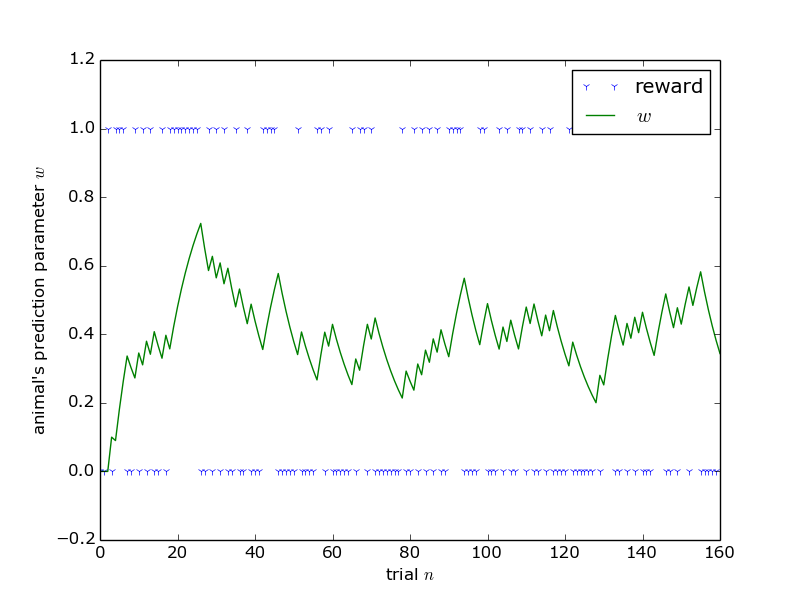
\includegraphics[width=0.7\linewidth]{pavCond4}
  \caption {Evolution of $w$ in the partial conditioning experiment 
            ($p = 0.4$, $\epsilon = 0.1$)}
\end{figure}

We can see that the curve becomes quite noisy because the experiment is not
deterministic anymore, but roughly speaking, $w$ tends to increase at the
beginning and then oscillates around 0.4. However, its value will never
converge. As a matter of fact, the learning rate $\epsilon = 0.1$ is too high
and a small number of trials can affect the animal's prediction parameter. 
We can redo the same simulation but with other $\epsilon$ values and over more
trials to be able to see the evolution of $w$ for smaller learning rate.

\vspace{-1em}
\begin{figure}[H]
  \centering
  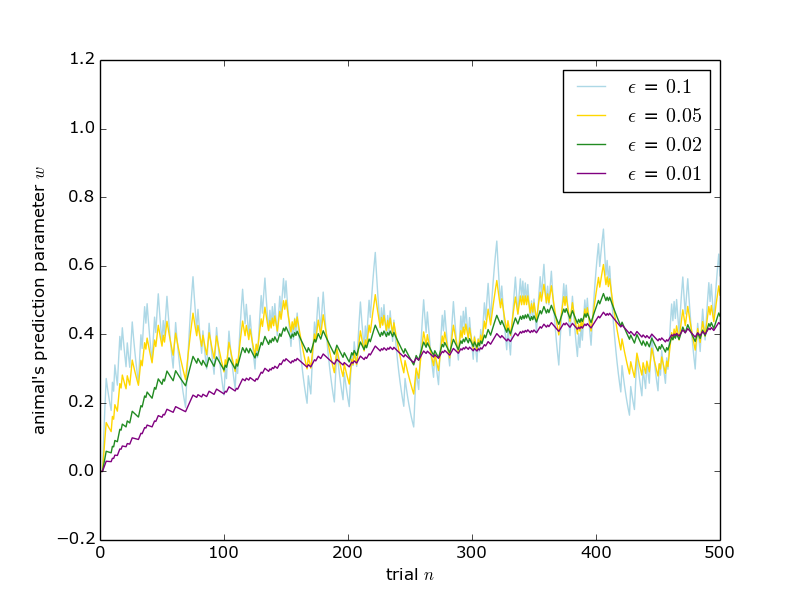
\includegraphics[width=0.7\linewidth]{pavCond5}
  \caption {Evolution of $w$ in the partial conditioning experiment with 
            different $\epsilon$ ($p = 0.4$)}
\end{figure}

As predicted, when the learning rate decreases, in particular when it equals 
0.01, it takes more time for the animal to learn, but the final value is also
more stable and doesn't deviate very much from 0.4. On the contrary, we can
imagine that if $\epsilon$ is bigger than 0.1, the curve becomes even noisier
and one can never learn the probability value $p = 0.4$, which 
confirms what is said before.

\subsection{Blocking effect}

Another advantage of the Rescola-Wagner model is that it allows us to explain
the blocking effect. It means that the conditioning of an association between
a CS and an US can be impaired if during the conditioning process, the CS is 
presented together with another CS that is already associated with the US. 
Therefore, in the newer experiment, we need two stimuli CS1 and CS2. In the 
first 25 trials, only CS1 and the reward (US) are present, and during the next
25 trials, CS1, CS2 and the reward are all present. We choose as usual 
$\epsilon = 0.1$. 

\vspace{-1em}
\begin{figure}[H]
  \centering
  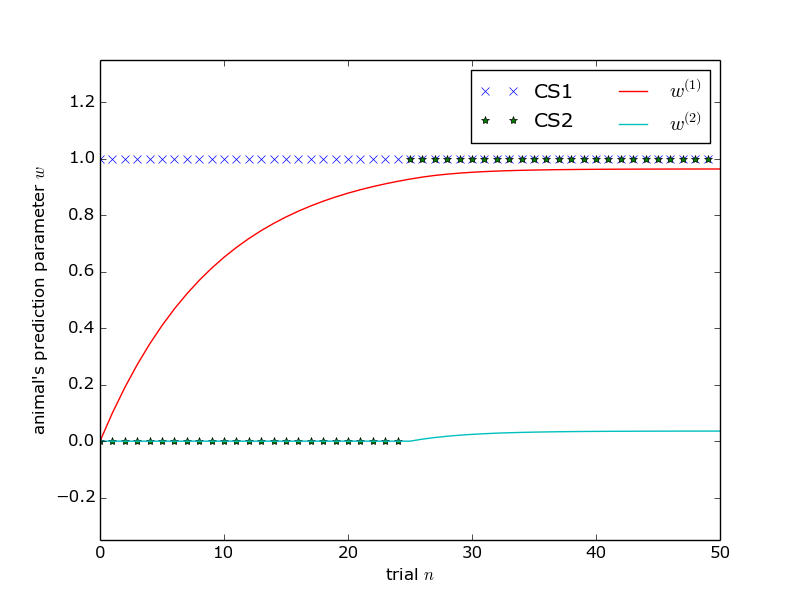
\includegraphics[width=0.7\linewidth]{pavCond6}
  \caption {Simulation of the blocking effect ($\epsilon = 0.1$)}
\end{figure}

We get the expected result: the conditioning of CS2 is blocking by the 
presence of CS1.  In the R-W model, the blocking effect can be explained
by the fact that $\delta = r - v = r - w^{(1)} - w^{(2)}$ is small during the
last 25 trials and using the update rule 
$w_{t+1}^{(2)} = w_t^{(2)} + \epsilon\delta_t u_t^{(2)}$ we can hardly change 
the value of $w^{(2)}$.

\subsection{Overshadowing}

In reality, there is no reason to assume that $\epsilon$ is the same for all
the stimuli. We should replace the global $\epsilon$ by some individual 
$\epsilon^{(i)}$ for each $i$. Then, in order to compare different 
$\epsilon^{(i)}$, a simple experiment can be considered: all the stimuli and 
the reward are all the time present and we just need to see which particular 
stimulus is the most associated with the reward after a certain number of 
trials. For example, if we use two stimuli CS1 and CS2 with respective 
learning rate 0.2 and 0.1, we plot the result as below.

\vspace{-1em}
\begin{figure}[H]
  \centering
  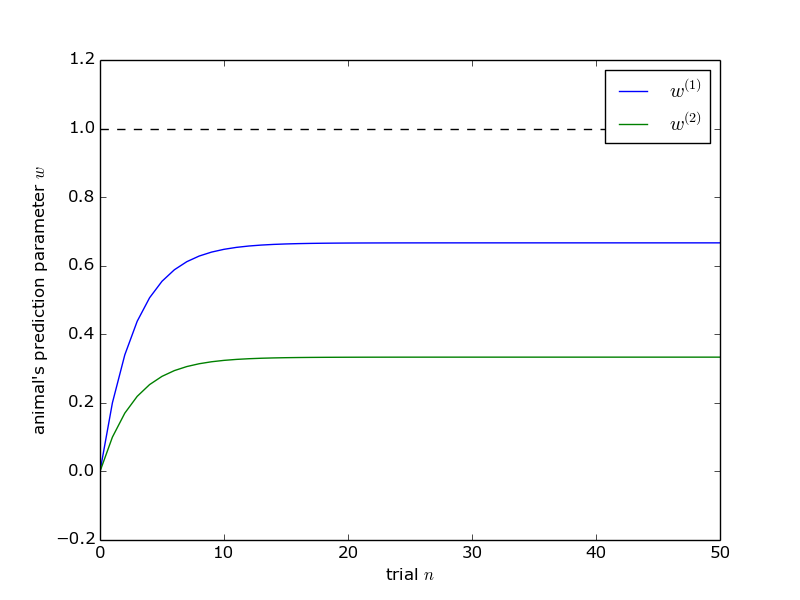
\includegraphics[width=0.7\linewidth]{pavCond7}
  \caption {Simulation of the overshadowing effect 
            ($\epsilon^{(1)} = 0.2$, $\epsilon^{(2)} = 0.1$)}
\end{figure}

The stimulus with a higher learning rate (in this case CS1) is more associated
with the reward. And if the difference between two learning rates become even
larger, it can result in a very weak conditioning of CS2. This is known as the 
overshadowing effect. We note that neither of the stimuli is fully associated
with the reward, but if we add $w^{(1)}$ and $w^{(2)}$, we get something very
close to 1.

\subsection{Conclusion}

In the Rescola-Wagner model conditioning means learning association between
conditioned and unconditioned stimuli. At the beginning, we saw that
this model could help us understand how one gets conditioned by a stimulus and 
how this conditioning can again disappear. The most appropriate value of the
learning rate may vary from case to case. Next, it turned out that even in a
non-deterministic experiment the model is able to find the key probability 
value. Blocking and overshadowing can also be explained. 

Of course this simple model has its limit. For instance, high-order 
conditioning requires us to take into consideration the time factor, which is
not done yet for the time being. Nonetheless, this model is not totally absurd
either. In fact, studies have suggested that the activity of some dopaminergic 
neurons in the brain encodes effectively the prediction error $\delta$ of the
model.


\section{Operant conditioning}

\subsection{Model description}

Operant conditioning is also called instrumental conditioning. It differs from
classical conditioning in that the acquired reward or punishment is mainly
decided by the agent's behavior, so what one needs to learn is the association
between each behavior and its consequence.

We'll illustrate this idea through a small example here. A bee is collecting
nectar from yellow and blue flowers, and at every moment, each type of 
flower carries a specific reward, which is denoted by $r_b$ for blue flowers
and $r_y$ for yellow ones. However, the bee is not aware of the exact values
of nectar rewards. Instead, it has some internal estimates $m_b$ and 
$m_y$. What the bee needs to do is therefore to make decisions on the basis
of these two values and to do real-time updates of them using what it knows.

\subsection{Softmax strategy}

For the decision part, we assume that the bee adopts the softmax strategy.
That is, it chooses the flower of type $i$ with probabily 

\[p_i = \frac{\exp(\beta m_i)}{\exp(\beta m_y) + \exp(\beta m_b)}\]

\noindent
where $i \in \{b, y\}$ and $\beta$ is the ``expoitation-exploration
trade-off" parameter (or the inverse temperature parameter if we refer to
the Boltzmann distribution model). Writing in this form, it can be easily
generalized to situations with more than two types of flowers, but we can also
write, for example for $p_b$

\[p_b = \frac{1}{1 + \exp(\beta(m_y - m_b))}.\]

The name of $\beta$ comes from the fact that it controls the bee's attitude
towards explorative and exploitative behavior. To see this, we can fix 
$m_y - m_b$ and plot $p_b$ as a funcion of $\beta$.

\vspace{-1em}
\begin{figure}[H]
  \centering
  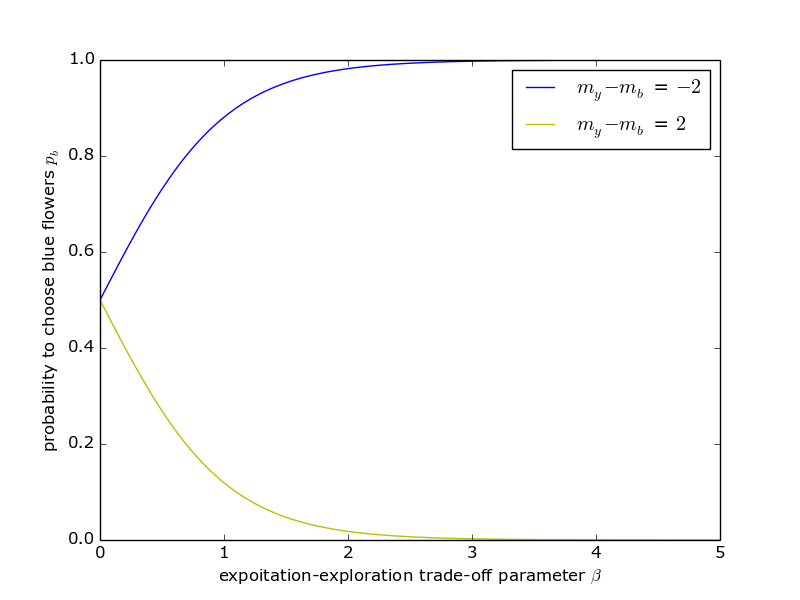
\includegraphics[width=0.7\linewidth]{insCond1}
  \caption {Plot of $p_b$ as a funcion of $\beta$ with fixed $m_y-m_b$}
\end{figure}

When the difference $m_y - m_b$ is positive, yellow flowers are more rewarding
to the bee than blue flowers, so generally speaking it tends to go to
yellow flowers to collect nectar. This tendancy is however not very clear when
$\beta$ is small, it suggests that the bee doesn't trust very much its own
estimates and puts emphasis on the exploration side. 

On the other hand, when
$\beta$ gets larger (in this case typically when it's greater than 2), the bee
goes to yellow flowers almost all the time. This implies the bee exploits a
lot what it has learned and doesn't explore much. Now if $m_y - m_b$ is
negative, it means that blue flowers are more attractive to bees so the two
curves are horizontally symmetrical but the effect of $\beta$ is the same.
We can also plot $p_b$ as a function of $m_y - m_b$ by fixing $\beta$.

\vspace{-1em}
\begin{figure}[H]
  \centering
  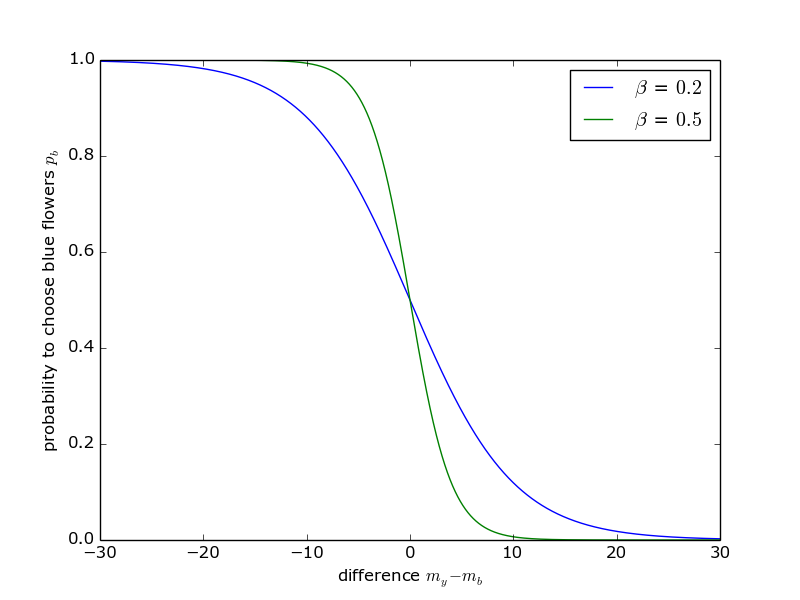
\includegraphics[width=0.7\linewidth]{insCond2}
  \caption {Plot of $p_b$ as a funcion of $m_y-m_b$ with fixed $\beta$}
\end{figure}

It's not surprising to get some sigmoid curves whose steepness depends on
parameter $\beta$. When $m_y - m_b$ tends to minus infinity, $p_b$ tends 
to 1 because the bee believes that blue flowers are much better than their 
yellow counterparts, and when $m_y - m_b$ tends to plus infinity, $p_b$ tends 
to 0 (here we're supposing implicitly $\beta > 0$).

\subsection{Dumb bee}

Before discussing how to update estimated rewards, we'll first do some
simulations with the policy given in the last paragraph. The simulation is for
two days. During the fisrt day we have $r_b = 8$ and $r_y = 2$. During the
second day, they're set to $r_b = 2$ and $r_y = 8$. The bee is able to sample
100 flowers during one day. Throughout the simulation, the bee can never learn
and believes that $m_y = 5$ and $m_b = 0$. First let's assume $\beta = 0$.

\begin{figure}[H]
  \centering
  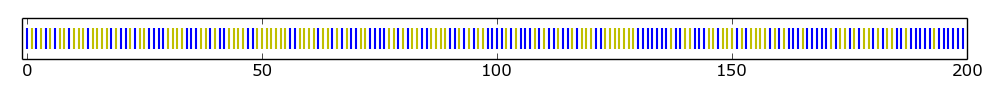
\includegraphics[width=1\linewidth]{insCond3}
  \caption {The choice of the dumb bee for 200 samplings during two days, 
            $\beta = 0$}
\end{figure}

It's known that when $\beta = 0$ the bee chooses blue and yellow
flowers equiprobably regarless of its internal estimates. This is indeed what
is observed here, it's not obvious to say the bee goes to blue or yellow
flowers more often (naturally, blue bars for blue flowers and yellow bars for
yellow flowers). We do one more simulation with this time $\beta = 0.8$.

\begin{figure}[H]
  \centering
  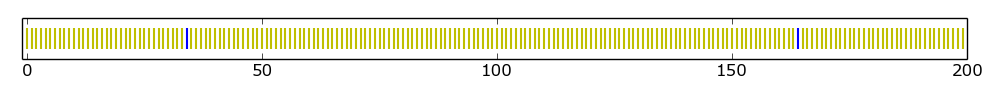
\includegraphics[width=1\linewidth]{insCond4}
  \caption {The choice of the dumb bee for 200 samplings during two days, 
            $\beta = 0.8$}
\end{figure}

In this case using the given formula we have $p_b = 1/(1 + e^4) \sim 1.7\% $.
Our result of the simulation is not very far from this value. The bee visits
blues flowers only twice which stands for a probability of 1\%. Anyway, in the
two cases, we can say that the bee's performance is quite poor because it
doesn't learn from experiences, in average the reward that the bee gets is 5
but it could have done better.

\subsection{Smart bee}

To learn the estimated reward, we inspire from the first part of the report,
the R-W model. Consequently, the online update rules are given by

\begin{gather*}
  m_b \rightarrow m_b + \epsilon(r_b - m_b)\\
  m_y \rightarrow m_y + \epsilon(r_y - m_y)
\end{gather*}

where as usual $\epsilon$ is the learning rate. The first rule is only used
when the bee visits a blue flower and similarly the second rule is considered
only when it visits a yellow flower. We start again from $m_y = 5$, $m_b = 0$
and we give $\epsilon = \beta = 0.2$.

\begin{figure}[H]
  \centering
  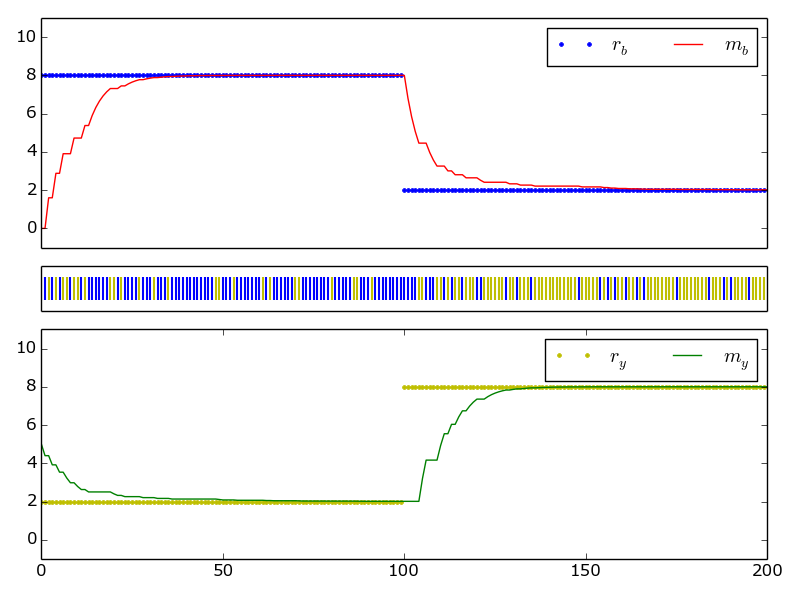
\includegraphics[width=0.7\linewidth]{insCond5}
  \caption {Smart bee's choices and internal estimates over two days with 
            $\epsilon = \beta = 0.2$}
\end{figure}

For the bee this is rather a satisfying result. It's able to learn correctly
the reward values and it can also take advantage of what it learns. On average
it gets almost 8 units of reward per trial, which is optimal. We will
then look at some extreme cases, such as the purely explorative behavior with
$\beta = 0$ and the case of strongly exploitative behavior with $\beta=1$.

\begin{figure}[H]
  \centering
  \begin{subfigure}[]{0.45\textwidth}
    \centering
    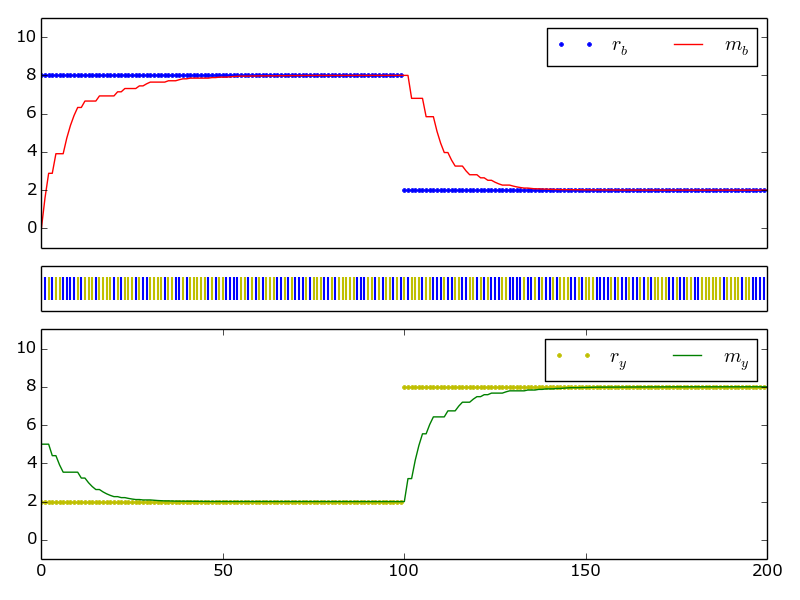
\includegraphics[width=\linewidth]{insCond6}
    \caption{$\beta = 0$}
  \end{subfigure}
  \begin{subfigure}[]{0.45\textwidth}
    \centering
    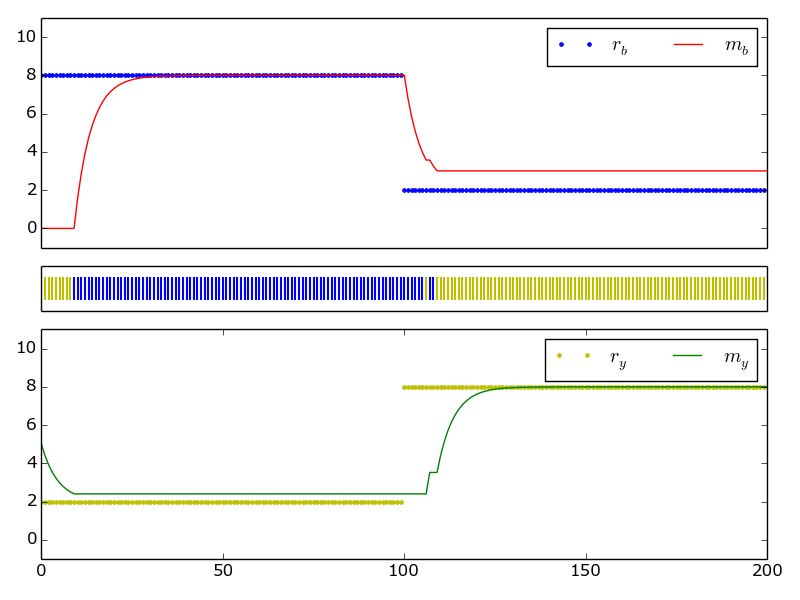
\includegraphics[width=\linewidth]{insCond7}
    \caption{$\beta = 1$}
  \end{subfigure}

  \caption {Smart bee's choices and internal estimates over two days with 
            $\epsilon = 0.2$}
\end{figure}

For $\beta = 0$, in terms of estimated reward the real value can be learned so 
it works correctly. Nonetheless, if we take a look at the bee's choices, it's 
completely random and it doesn't benefit at all from what it has learned.

On the other hand, when $\beta = 1$, surprisingly the outcome is quite ideal. 
In reality, at the beginning of the two days, the bee learns that the real 
reward that yellow/blue flowers carry is only 2 so it would also give a try to
the other kind of flowers and it discovers that it's pretty appealing. 
However, we can also imagine a scenario where in the second day the blue 
flowers have always almost the same amount of nectar but the nectar that one 
yellow flower carries gets even higher.

\begin{figure}[H]
  \centering
  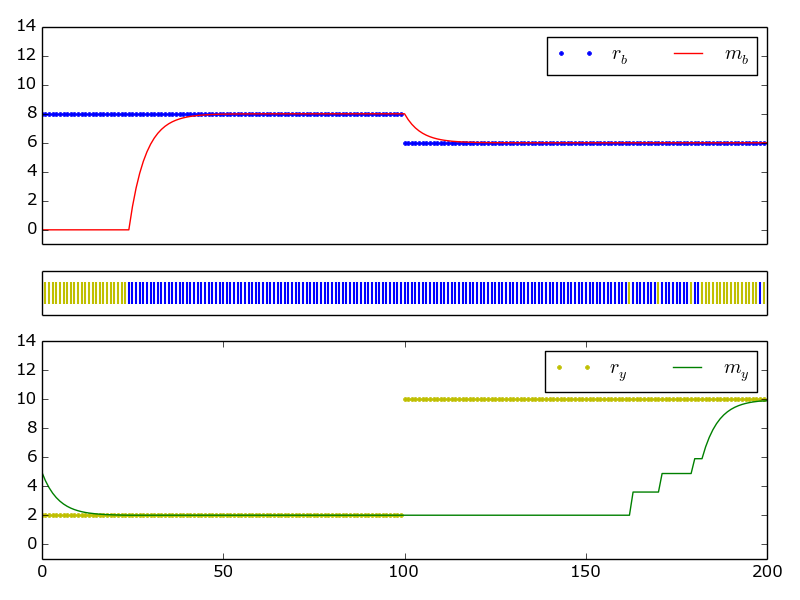
\includegraphics[width=0.7\linewidth]{insCond8}
  \caption {Smart bee's choices and internal estimates over another two days 
            with $\epsilon = 0.2$, $\beta = 1$}
\end{figure}

We see that if the bee is lucky it may be able to learn correctly $r_b$ and
$r_y$, but it takes quite a long time because
the bee goes very rarely to the type of flowers that it estimates  not
rewarding. As a consequence, it can hardly benefits from this change.

\begin{figure}[H]
  \centering
  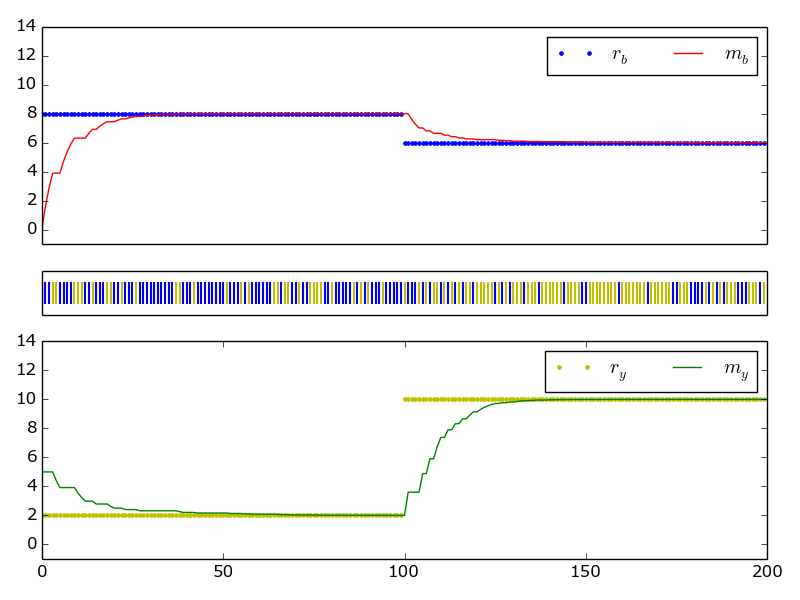
\includegraphics[width=0.7\linewidth]{insCond9}
  \caption {Smart bee's choices and internal estimates over another two days 
            with $\epsilon = \beta = 0.2$}
\end{figure}

On the contray, if we come back to the initial value of $\beta$ the bee 
becomes quickly aware of the modification and can therefore take advantage of
it. 

\subsection{Conclusion}

In operant conditioning the agent needs to make choices in order to receive 
the corresponding award or punishment. So the reward value is now associated 
with each action. In addiction to learn these values, one also needs to carry
out its actions according to its internal estimates. The softmax strategy is 
often considered for the policy part. It seems rational, but the agent must 
adapt its $\beta$ parameter to the environment and finds a trade off between 
explorative and exploitative behavior. The delta rule is again used for the 
learning part. By combining these two sides with some adequate parameter 
values, the agent is able to make nice reponses to environmental changes.


\section{Drift diffusion model}

\subsection{Model description}

In a two-alternative forced task (2AFC-task), subjects are asked to choose
between two alternative actions. For example, we can consider that the subject
is looking at a set of dots on a screen that are moving in different
directions and needs to indicate whether they're moving upwards or downwards.
A stimulus can be very noisy. In such case, only a small part of the dots
are moving in the right direction and the other points move randomly. 

Then one way to describe the decision-making process is the drift-diffusion
model. We assume that the subject is accumulating evidence for one or other of
the alternatives at each time step. In our example, the subject compares the
firing rate $m_A$ of an upward-motion sensitive neuron with the firing rate 
$m_B$ of an downward-motion sensitive neuron. From this, it computes an
integration variable $x$ that obeys 

\[\dot{x} = m_A - m_B + \sigma\eta(t)\]

\noindent
where $\eta(t)$ is a noise term (Guassian white noise with unit standard
deviation) simulating the noisiness of real neurons and $\sigma$ represents 
the noise level. If $x$ surpasses a threshold $\mu$, the subject decides for 
outcome $A$; on the contrary, if $x$ gets lower than $-\mu$, the subject 
decides for outcome $B$. To compute  $x$ in our program, we simply use the 
Euler method 

\[x(t+\Delta t) = x(t) + (m_A - m_B)\Delta t + 
  \sigma\tilde{\eta}(t)\sqrt{\Delta t}\]

\noindent
where $\tilde{\eta}(t)$ is selected randomly from a standard Gussian 
distribution.

\subsection{Evolution of $x$}

We'll thus simulate the decision-making process by computing the evolution of
$x$. We choose $m_A = 1$, $m_B = 0.95$, $\Delta t = 0.1$ms, $\sigma = 1/2$,
$\mu = 0.4$ and finally $x(0) = 0$ (the subject is neutral at the beginning of
the experiment). The simulation is run until $t = 1$s.

\vspace*{-1em}
\begin{figure}[H]
  \centering
  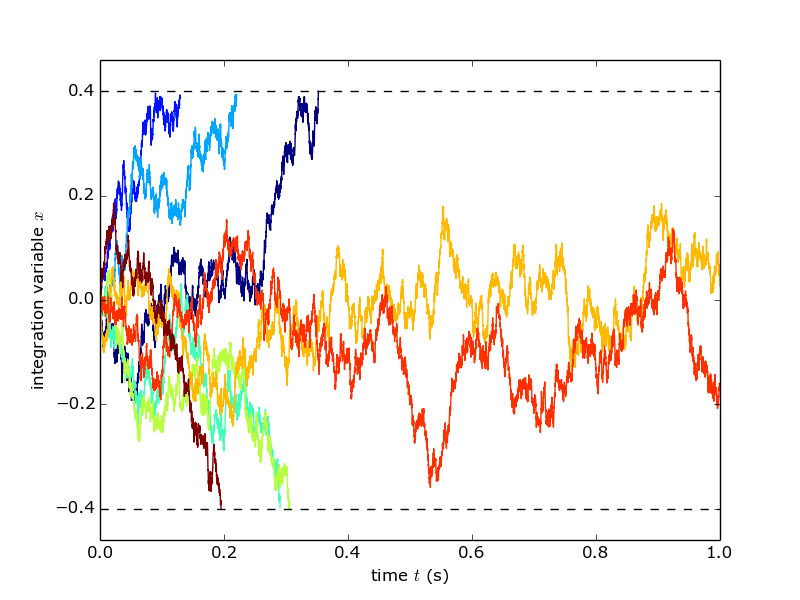
\includegraphics[width=0.7\linewidth]{Drifdiff1}
  \caption {Eight runs of the drift diffusion model}
\end{figure}

The curves are very noisy and even though $m_A > m_B$, the subject chooses B 
as the final outcome quite often; it's not clear that the probability of
choosing A is really higher here. It's simply because $m_A$ is very close to
$m_B$ in this case and more simulations are needed to do a deeper analysis.  
We also see that the subject may not be able to make the decision by the time
$t = 1$s.

\subsection{Reaction time}

We are now intrested in the reaction time of the subject. If $x$ cross the
threshold at time $t_i$, we claim that the reaction time of this run is
$\mathrm{RT}_i = 100 + t_i$ (take into consideration the time that is needed 
for the nerve signal to be transmitted). We'll then do the simulation 1000 
times to see the distribution of reactions times for outcome A and for outcome
B.

\begin{figure}[H]
  \centering
  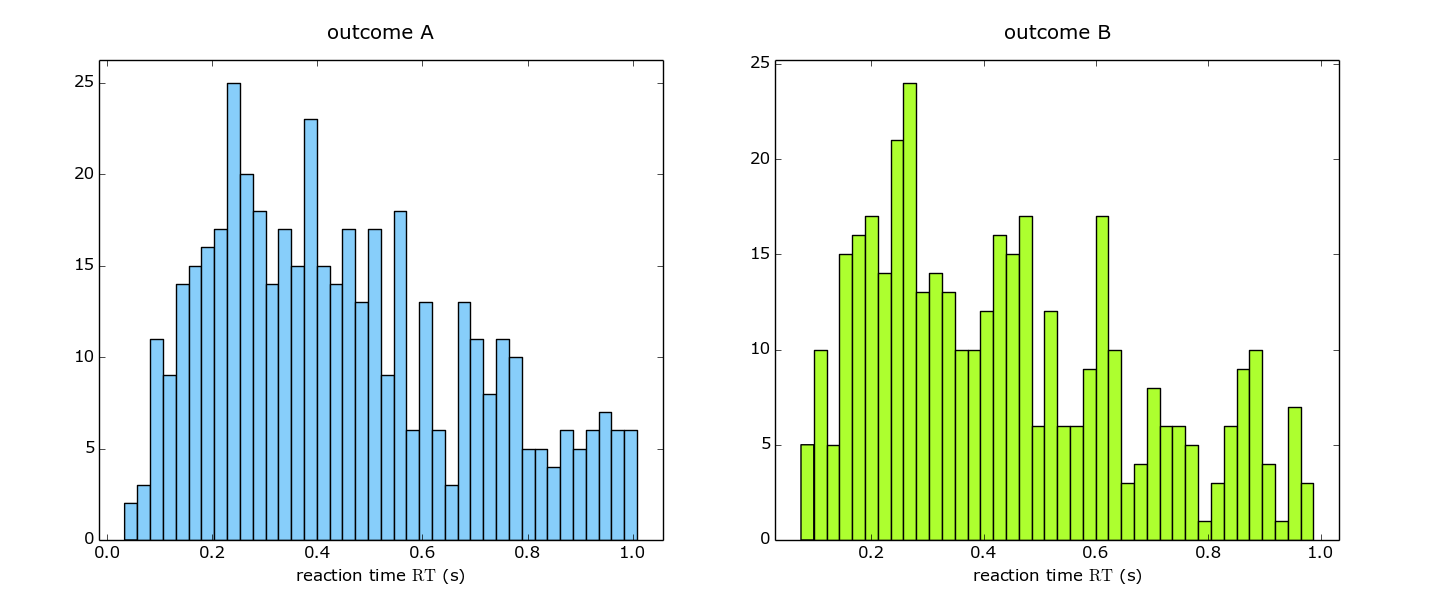
\includegraphics[width=\linewidth]{Drifdiff2}
  \caption {Distribution of reaction times}
\end{figure}

The two histograms have quite similar patterns. It might not be evident to 
find an exact function to describe the distibution, but at least we observe 
that decisions are the most often made at the early stage of the simulation 
(between 0.2 and 0.4s). In addition, with 1000 simulations, we can also see
that A is more often chosen than B. In fact, in the above figure, A is chosen
453 times while B is chosen only 389 times (we notice that naturally the
sum is not 1000 due to what is mentioned in the last paragraph).

\subsection{Probability of choosing a specific outcome}

We now denote the evidence for outcome A versus outcome B as $m_E = m_A - m_B$.
It's intuitive that when $m_E$ gets larger, the probability $p_A$ of choosing 
A as outcome also increases. In reality, we have the analytical formula

\[p_A = \frac{1}{1 + \exp(\beta(m_B - m_A))}\]

\noindent
where $\beta = 2\mu/\sigma^2$. To deduce the probability value by using
computer simulations, for a fixed $m_E$, we'll carry out the simulation 1000 
times to calculate the corresponding $p_A$. We plot the probabilities computed
in this manner as a function of $m_E$ for $m_E$ ranging from -0.2 to 0.2. The
result is shown at the top of the next page.

Even though it's not yet perfect, the simulation result follows globally the
given formula. We can imagine that when the number of simulations used to
caclulate the probability tends to infinity, the simulation curve will 
converge to the theoretical one.

\vspace*{-1em}
\begin{figure}[H]
  \centering
  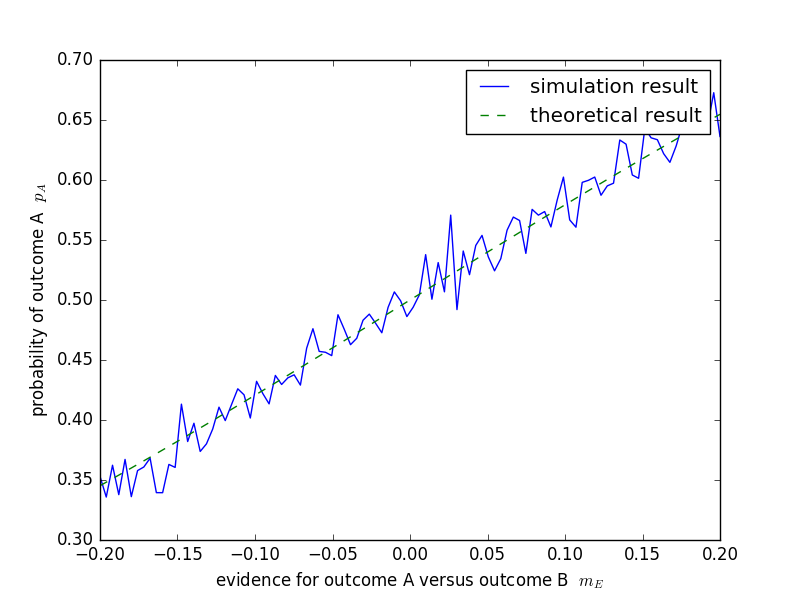
\includegraphics[width=0.7\linewidth]{Drifdiff3}
  \caption {Probability of choosing A for different values of $m_E$}
\end{figure}

\subsection{Conclusion}

Many models are proposed to explain experimental data for 2AFC tasks. DDM is
just one of them. The model suggests that the subject is accumulating evidence
from the past to make decisions and simulation results seem to match real
observations in terms of both external behaviors and neuron activities. As a
matter of fact, in the task that is mentioned here, the lateral intraparietal
area (LIP) of parietal cortex involved in saccadic movements (we ask the
subject to respond by making a saccade to the location of the target) may have
neurons that are somehow doing what is described in the model. 


\section{Temporal difference (TD) learning}

\subsection{Model description}

In a reinforcement learning problem an agent needs to act in the world to
maximize its rewards. It's a little like the operant conditioning problem that
we've discussed in the second part, but now the time dimension is integrated 
and the reward is thus no longer immediate. In a way, the agent must be able to
``predict the future" to perform the right sequence of actions.

We consider for example a simple maze navigation problem. A rat enters a
maze having 7 states $\{A,B,C,D,E,F,G\}$. It starts always at state $A$, it 
can then moves on to either state $B$ or $C$. At $B$ it can go to either $D$ 
or $E$ and when it's at $C$, $F$ and $G$ are accessible. Among all of these 
states, only states $E$ and $F$ are rewarding, with respectively 5 and 2 
units of reward. Finally, the rat is taken out of the maze by the 
experimenter, and thereby moves into the ``terminal" state $H$.

\subsection{Just be random}

To make things easier, the rat can of course adopt a totally random stategy.
Every time when it is at a junction, it goes to either left or right 
with 50\% probability. Now if we do 100 simulations, theoritically, 
the number of times it visits each state will be: 100 for $A$ and $H$, 50 for 
$B$ and $C$, and 25 for the rest. What we actually get is:

\vspace{0.5em}
\begin{table}[h]
  \tabcolsep = 16pt
  \caption
    {Number of visits for each state in 100 trials with a random strategy}
  \begin{tabular*}{\linewidth}{>{\it}lcccccccc}
    \toprule
    State & $A$ & $B$ & $C$ & $D$ & $E$ & $F$ & $G$ & $H$ \\ 
    Number of visits & 100 & 51 & 49 & 28 & 23 & 22 & 27 & 100 \\
    \bottomrule
  \end{tabular*}
\end{table}

That is not very far from the theoritical value. Next, we want to associate a
value with each state, which will be evaluated as the expected sum of all
possible future rewards when the rat is at this state. While the rat is 
carrying out the experiment, we want to update these values as well. This can 
be done through the temporal difference learning rule

\[V(s_t) \leftarrow V(s_t) + \epsilon[r(s_t)+V(s_{t+1})-V(s_t)]\]

\noindent
where $s_t$ with $t = \{1,2,3,4\}$ denotes the sequence of states in a trial.
The idea is that the reward that the rat is meant to get at $s_t$ is 
$V(s_{t+1}) - V(s_t)$ and we apply just the delta rule. The update is 
performed after each trial.

\vspace*{-1em}
\begin{figure}[H]
  \centering
  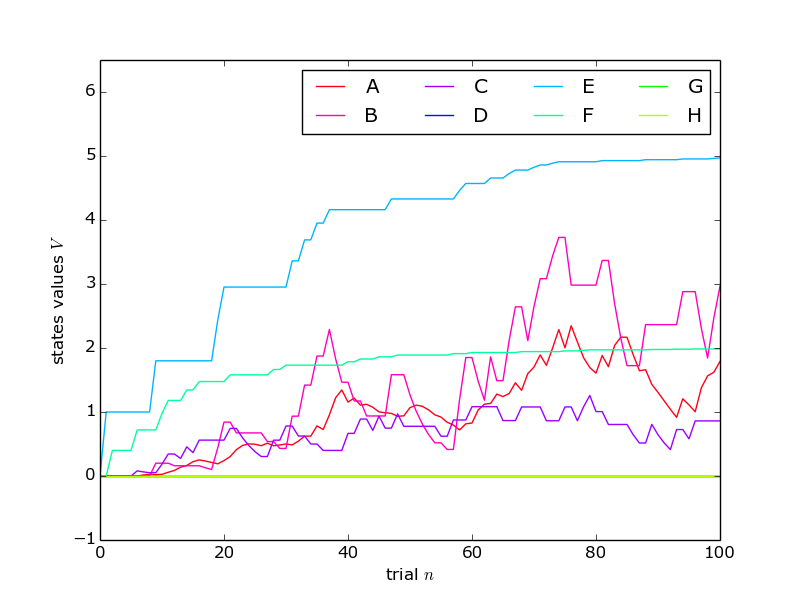
\includegraphics[width=0.7\linewidth]{TDlear1}
  \caption {Evolution of state values using a random strategy}
\end{figure}

The rat manages to learn correctly the state values. For example we indeed
obtain $V(E) \sim 5$ and $V(F) \sim 2$. Notice that $B$ is not as valuable as 
$E$ even though one can choose deterministically to go to $E$ at $B$. This is
simply due to the fact that the rat is using a random strategy. In a similar
way, $C$ is not as valuable as $F$. We'll see later that if the rat chooses
almost surely to go to the side with the larger value, the result will be
different.

\subsection{And softmax again}

Now that we're able to learn the state values, we'll study a more complicated
way to make decisions. There is nothing new, at each junction, the rat chooses
which state to go using the softmax strategy.
We'll first pick up a quite neutral value of $\beta$, 
say, $\beta = 0.3$. As the purely explorative behavior is exactly the same
thing as the random strategy, instead of $\beta = 0$ we'll choose 
$\beta = 0.05$ to have another example of highly explorative behvaior.

\vspace*{-0.2em}
\begin{figure}[H]
  \centering
  \begin{subfigure}[]{0.45\textwidth}
    \centering
    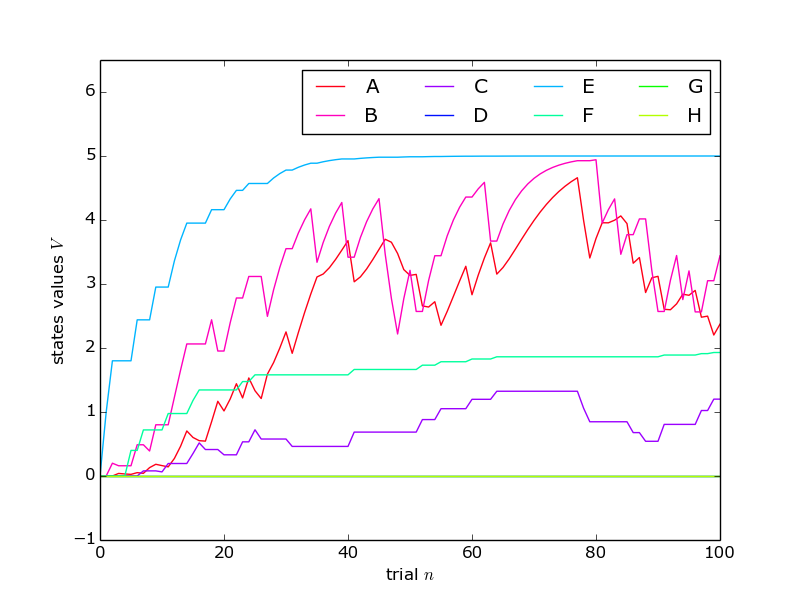
\includegraphics[width=\linewidth]{TDlear3}
    \caption{$\beta = 0.3$}
  \end{subfigure}
  \begin{subfigure}[]{0.45\textwidth}
    \centering
    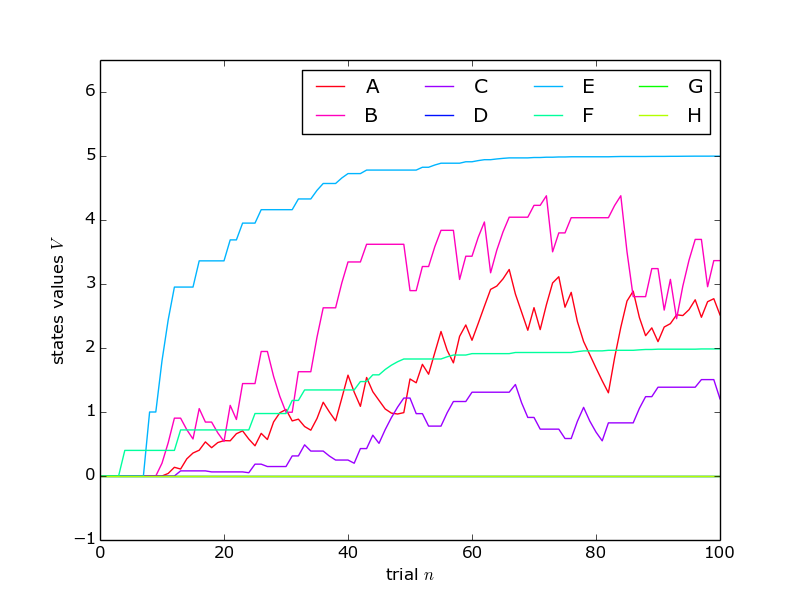
\includegraphics[width=\linewidth]{TDlear2}
    \caption{$\beta = 0.05$}
  \end{subfigure}

  \caption {Evolution of state values using the softmax strategy}
\end{figure}

Naturally, the rat succeeds in learning the right values. $V(A)$ and $V(B)$ 
are higher than before. Moreover, we know that by using the softmax decision
rule the rat benefits from its own knowledge. It's shown in the table below,
the rat reaches state $E$ much more often.

\vspace{0.5em}
\begin{table}[h]
  \tabcolsep = 16pt
  \caption
    {Number of visits for each state in 100 trials with a softamx strategy,
    $\beta = 0.3$}
  \begin{tabular*}{\linewidth}{>{\it}lcccccccc}
    \toprule
    State & $A$ & $B$ & $C$ & $D$ & $E$ & $F$ & $G$ & $H$ \\ 
    Number of visits & 100 & 75 & 25 & 17 & 58 & 15 & 10 & 100 \\
    \bottomrule
  \end{tabular*}
\end{table}

\vspace{0.3em}
\noindent
What if the rat is very greedy? We assume that $\beta = 1$.

\vspace*{-1em}
\begin{figure}[H]
  \centering
  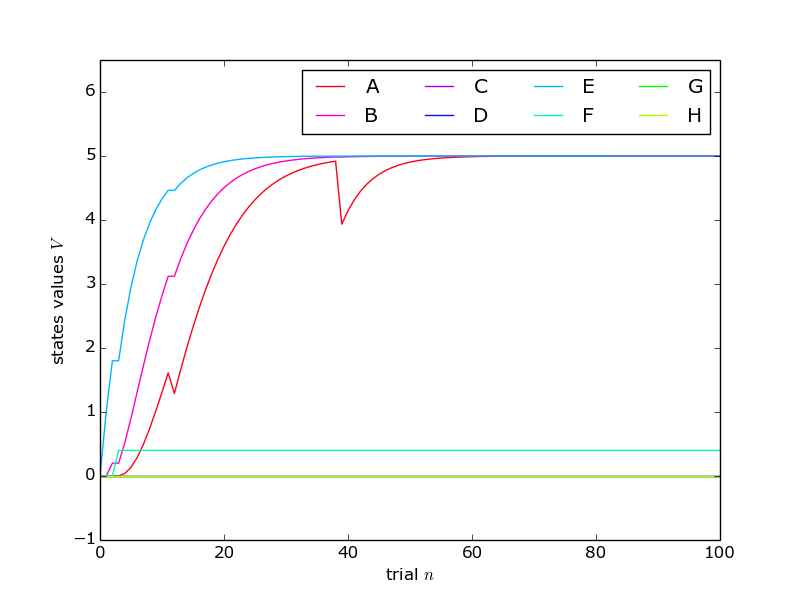
\includegraphics[width=0.7\linewidth]{TDlear4}
  \caption {Evolution of state values using the softmax strategy, $\beta = 1$}
\end{figure}

As promised before, both state $A$ and $B$ are as valuable as state $E$ 
because the rat will almost always chooses to go to $E$ when it's on these two
states. We might also note that the rat never learns the correct value of 
$V(F)$. It doesn't really matter here since $E$ provides more reward than $F$,
but we can also imagine that if very unluckily, at the beginning of the
experiment, the rat gets to $F$ a lot of times, it may learn $V(F) = 2$ while 
$V(E)$ is still zero and then decides to go to $F$ all the time. Generally
speaking, being too exploitative/greedy prevents the agent from learning new
things and decreases its adaptability to environment changes.

\subsection{Conclusion}

In this final section, we have worked on a simple maze navigation problem and
tried to solve it using TD learning. The key point is to represent all the
future possible rewards as the value of each state to allow us to have a
long-term consideration. 

We didn't take into account the discount factor which supposes that 
the future doesn't have the same worth as the present. Other similar 
techniques include Q learning and SARSA that combines states and actions and
give values to each possible couple $(state, action)$. Nevertheless, all of
them share the same idea: in these values we integrate the present and the
future, and in each new trial they're updated to take into consideration the 
newest information.
